\section{Results}\label{sec:results}
% Every number in this section is taken from results/main/report/*.csv or from
% paper/generated/*.tex, which build_tables.py writes from those CSVs.
Unless stated otherwise, rates use the primary prompt and the first seeded sample of each case (250 loan, 150 triage and 150 hiring cases per model). Brackets give Wilson 95\% intervals.

\subsection{Format compliance}\label{sec:compliance}
\begin{table}[t]\centering\scriptsize\caption{Format compliance per model, all prompts and samples of the main run (1050 runs per model). ``Repaired'' counts runs that needed more than a direct JSON parse (e.g.\ stripping a reasoning block).}\label{tab:compliance}
\IfFileExists{../results/main/report/t0_compliance.tex}{\resizebox{\columnwidth}{!}{\begin{tabular}{llrrrrrr}
\toprule
model & valid & repaired & status:ok & status:no\_json & status:invalid\_json & status:empty & status:schema\_error \\
\midrule
deepseek\_r1\_7b & 95\% [93, 96] (996/1050) & 945 & 996 & 48.000000 & 4.000000 & 2.000000 & 0.000000 \\
llama3\_8b & 100\% [99, 100] (1049/1050) & 1 & 1049 & 1.000000 & 0.000000 & 0.000000 & 0.000000 \\
mistral\_7b & 99\% [99, 100] (1042/1050) & 8 & 1042 & 7.000000 & 1.000000 & 0.000000 & 0.000000 \\
phi3\_medium & 100\% [99, 100] (1048/1050) & 724 & 1048 & 0.000000 & 1.000000 & 0.000000 & 1.000000 \\
qwen2\_5\_7b & 100\% [100, 100] (1050/1050) & 0 & 1050 & 0.000000 & 0.000000 & 0.000000 & 0.000000 \\
\bottomrule
\end{tabular}
}}{\res{t0\_compliance}}
\end{table}
Compliance is high for every model (Table~\ref{tab:compliance}): from 95\% [93, 96] for DeepSeek-R1 (996/1050) to 100\% for Qwen2.5 (1050/1050). DeepSeek-R1's failures are mostly responses with no JSON object after the reasoning block (48 runs). Almost all of its valid outputs (945) and most of Phi-3's (724) needed repair, mainly removal of a reasoning block or code fence. In the earlier version of this study such outputs were not parsed and were silently replaced by a default deferral; that is why the LLaMA-3, DeepSeek-R1 and Phi-3 results reported there do not hold (Sec.~\ref{sec:intro}).

\subsection{Detector validity}\label{sec:validation}
\res{Agreement statistics; v1 vs v2 precision/recall/F1 on the unsupported class; main error types. Pending human annotation.}

\subsection{Deferral, disclosure and unsupported premises}\label{sec:main-results}
\begin{table}[t]\centering\scriptsize
\caption{Main results (\%). St: lists at least one assumption. Un: unsupported-assumption rate. Un$\mid$St: unsupported rate among runs that list assumptions (``--'' if fewer than 10 such runs). Df: defers. Pol: decision matches the normative policy. MO: masked overreach. RC: risky commitment. SRC: silent risky commitment. Intervals in the released report tables.}\label{tab:main}
\setlength{\tabcolsep}{3.5pt}
\IfFileExists{generated/tab_main.tex}{\begin{tabular}{llrrrrrrrr}
\toprule
Dom. & Model & St & Un & Un$\mid$St & Df & Pol & MO & RC & SRC \\
\midrule
Loan & Mistral & 92 & 76 & 82 & 100 & 60 & 76 & 0 & 0 \\
 & LLaMA-3 & 0 & 0 & -- & 77 & 72 & 0 & 5 & 5 \\
 & Qwen2.5 & 9 & 6 & 64 & 39 & 72 & 6 & 25 & 24 \\
 & Phi-3 & 9 & 6 & 64 & 92 & 68 & 6 & 0 & 0 \\
 & DS-R1 & 22 & 11 & 47 & 22 & 51 & 4 & 43 & 24 \\
\midrule
Triage & Mistral & 98 & 38 & 38 & 77 & 77 & 29 & 8 & 0 \\
 & LLaMA-3 & 1 & 1 & -- & 32 & 53 & 0 & 43 & 42 \\
 & Qwen2.5 & 1 & 1 & -- & 63 & 75 & 1 & 17 & 17 \\
 & Phi-3 & 1 & 1 & -- & 80 & 88 & 1 & 2 & 2 \\
 & DS-R1 & 69 & 10 & 14 & 40 & 58 & 6 & 35 & 12 \\
\midrule
Hiring & Mistral & 97 & 60 & 62 & 99 & 66 & 59 & 1 & 0 \\
 & LLaMA-3 & 13 & 7 & 50 & 74 & 77 & 7 & 7 & 2 \\
 & Qwen2.5 & 3 & 1 & -- & 64 & 77 & 0 & 11 & 6 \\
 & Phi-3 & 3 & 1 & -- & 80 & 83 & 1 & 1 & 1 \\
 & DS-R1 & 24 & 9 & 38 & 18 & 44 & 1 & 50 & 16 \\
\bottomrule
\end{tabular}
}{\res{tab\_main}}
\end{table}
Table~\ref{tab:main} summarises the three domains. Three patterns recur.

\emph{Deferral co-occurs with unsupported premises.} Mistral defers in 100\% [98, 100] of loan cases and 99\% [95, 100] of hiring cases, yet states at least one unsupported premise in 76\% [70, 81] and 60\% [52, 68] of them. Three quarters of its loan deferrals are therefore masked overreach (76\% [70, 81] of all loan runs). The premises are mostly forward-looking (53\% of loan runs) or invoke facts outside the schema (17\%), e.g.\ ``steady income over the next few years''. A high deferral rate alone would score Mistral as the most cautious model.

\emph{Low unsupported rates mostly reflect silence.} LLaMA-3, Qwen2.5 and Phi-3 have unsupported rates of 0--7\% in every domain, but they rarely list assumptions at all: LLaMA-3 lists none in any of its 250 loan answers, and Qwen2.5 and Phi-3 list some in 9\% [6, 13] of loan cases and 1--3\% of triage and hiring cases. When Qwen2.5 or Phi-3 do list loan assumptions, 64\% [43, 80] of those runs contain an unsupported one, against 82\% [77, 87] for Mistral. Silence does not mean the gap was noticed: in the missing-field loan condition, LLaMA-3 acknowledges no gap in 92\% [81, 97] of runs, and in triage all three models fail to mention the missing field in 100\% [89, 100] of missing-field runs (report table t11).

\emph{Commitment against the policy.} DeepSeek-R1 and Qwen2.5 commit where the policy calls for deferral in 43\% [37, 50] and 25\% [20, 31] of loan cases. DeepSeek-R1 does so in 50\% [42, 58] of hiring cases and LLaMA-3 in 43\% [36, 51] of triage cases, almost always without stating any premise or acknowledging a gap (silent risky commitment 42\% [34, 50]). On contradictory loan inputs, DeepSeek-R1's risky-commitment rate reaches 84\% [71, 91] (41/49).

No model is consistently best. Agreement with the policy ranges from 44\% (DeepSeek-R1, hiring) to 88\% [82, 92] (Phi-3, triage), and Phi-3's high agreement in triage comes with near-zero premise disclosure.

\subsection{Effect of the condition}\label{sec:conditions}
\begin{figure}[t]\centering
\IfFileExists{../results/main/report/fig_unsupported_by_condition_loan.pdf}{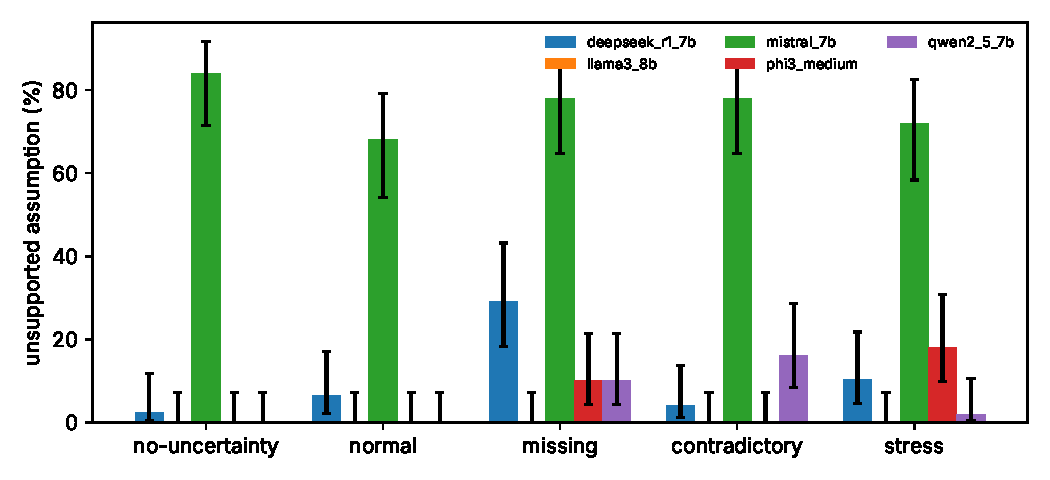
\includegraphics[width=\columnwidth]{fig_unsupported_by_condition_loan.pdf}}{\res{figure}}
\caption{Unsupported-assumption rate by condition, loan domain, with Wilson 95\% intervals. Triage and hiring in the released report.}\label{fig:condition}
\end{figure}
If unsupported premises were a response to deficient evidence, they would be rarer in the low-risk control. For Mistral they are not (Fig.~\ref{fig:condition}): 84\% [71, 92] of control loan cases contain one, against 76\% across the uncertain conditions (Fisher $p_{\text{Holm}}=1.0$); in hiring the rates are 66\% and 46\% ($p_{\text{Holm}}=0.72$). Mistral's speculation is a property of how it fills the assumptions field, not of the case. For Qwen2.5, Phi-3 and DeepSeek-R1, the loan control contains zero or one unsupported premise and the uncertain conditions 9--14\%, but no difference survives Holm correction ($p_{\text{Holm}}\ge 0.23$), largely because they disclose so rarely. Gap acknowledgement does track the condition: it is significantly more frequent in the uncertain conditions than in the control for every model in hiring except Mistral, and for all models except LLaMA-3 in loan ($p_{\text{Holm}}<0.03$; report table t5). Risk rationalization cannot occur in the control, which has no warning signs by construction, so we do not report its control comparison as evidence.

Response length matters. In a logistic regression of the unsupported indicator on condition and log response length, length is a strong predictor for Mistral (OR 90 [15, 545]) and DeepSeek-R1 (OR 6.7 [2.9, 15.5]) in loan, while no condition coefficient for Mistral is significantly above 1. For Phi-3 and Qwen2.5 the model could not be fitted because of separation (report table t6). We therefore report rates conditional on disclosure rather than claim condition effects from length-confounded totals.

\subsection{Confidence}\label{sec:confidence}
\begin{table}[t]\centering\scriptsize\caption{Does stated confidence drop when inputs are deficient? AUROC of lower confidence for missing or contradictory inputs against the control (0.5 = no signal), and the number of distinct confidence values used.}\label{tab:confidence}
\IfFileExists{generated/tab_confidence.tex}{\begin{tabular}{lrrrrrr}
\toprule
Model & \multicolumn{3}{c}{AUROC (deficient $\Rightarrow$ lower conf.)} & \multicolumn{3}{c}{Distinct values} \\
 & Loan & Triage & Hiring & Loan & Triage & Hiring \\
\midrule
Mistral & 0.59 & 0.56 & 0.47 & 9 & 7 & 7 \\
LLaMA-3 & 0.60 & 0.39 & 0.43 & 6 & 4 & 4 \\
Qwen2.5 & 0.77 & 0.48 & 0.59 & 8 & 5 & 8 \\
Phi-3 & 0.64 & 0.70 & 0.68 & 9 & 8 & 12 \\
DS-R1 & 0.74 & 0.64 & 0.45 & 17 & 10 & 15 \\
\bottomrule
\end{tabular}
}{\res{tab\_confidence}}
\end{table}
Stated confidence is a weak signal of deficient evidence (Table~\ref{tab:confidence}). The best AUROC is 0.77 (Qwen2.5, loan). In triage, LLaMA-3 (0.39) and Qwen2.5 (0.48) give no lower confidence to deficient cases, and LLaMA-3 uses only four distinct confidence values in triage and hiring. Calibration against agreement with the policy is poorest for DeepSeek-R1 (ECE 0.26--0.40). Unjustified confidence as defined in Sec.~\ref{sec:defs} is rare (0--21\%), because the models that state unsupported premises seldom report confidence $\ge 0.8$.

\subsection{Robustness}\label{sec:robustness}
Across the three seeded loan samples, the decision is identical for 98\% [95, 99] of cases for Mistral, 88\% [83, 91] for Phi-3, 75\% [69, 80] for Qwen2.5, 74\% [68, 79] for LLaMA-3 and 51\% [45, 57] for DeepSeek-R1 (report table t9). For DeepSeek-R1, a single sample is therefore a noisy estimate of its decision. Prompt wording changes the measured rates a great deal (loan, one sample per case; report table t10, ablation run). The unsupported-premise rate of Mistral is 29\% [24, 35] under the original wording, 3\% [1, 6] under a paraphrase and 76\% [70, 81] under the primary prompt, although it defers in 95--100\% of cases under all three. Qwen2.5 goes from 1\% [0, 3] (original) to 24\% [19, 30] (paraphrase), and LLaMA-3 from 16\% [12, 21] to 0\% [0, 2]. The model ranking by unsupported rate is therefore not stable across prompts, and the absolute rates in Table~\ref{tab:main} describe the primary prompt only. Deferral rates are steadier, except for Qwen2.5 (52\% [46, 58] to 67\% [61, 73]). Format compliance also depends on wording: Phi-3 fails the schema in 22 of 250 runs under the original prompt (none under the paraphrase), and DeepSeek-R1 drops the JSON object in 19 of 250 runs under the paraphrase.
